% Seminar work LaTeX-template for use in seminars in acoustics.
% Thanks go to Jussi Pekonen for editing and updating this template.

% Preferably use a combination of PdfTex and BibTex to compile. This
% can be done easily with a prepared package. Google is your help in
% this case.

% You can modify some things and add packages if you prefer. This setup,
% however, should be enough for most seminar papers. This has been tested
% with current version TeXLive-package (2010), which you should probably 
% use (MacTeX and MikTeX use it). If you do not want to use it, then

%
% Tapani Pihlajamäki 17.1.2011

% Set document class and encoding
\documentclass[11pt,a4paper,twoside]{article}
\usepackage[T1]{fontenc}

% Unicode input encoding
\usepackage{ucs}
\usepackage[utf8x]{inputenc}

% Language. Change to finnish if you write in finnish (or use both)
\usepackage[english]{babel}


% Microtype makes the text really neat.
\usepackage{microtype}

% Graphics package
\usepackage[pdftex]{graphicx}

% Package enabling subfigures. This means that you can use figures
% with automatic "numbering" and referencing.
\usepackage{subfigure}

% Extended equation and symbol functionality
\usepackage{amsmath}
\usepackage{amssymb}



% New fonts based on Aalto
\usepackage{fouriernc}
\usepackage[scaled]{helvet}
\renewcommand*\ttdefault{txtt}
%\usepackage{inconsolata}
\usepackage{tgheros}

% NatBib load. Check NatBib reference with Google if you want to know more
% about its options. In short, it is possible to modify almost everything
% about the citation style.
%\usepackage[round]{natbib}
\usepackage{cite}

% Acoustics style file.
\usepackage{akuseminar}

% Formatting for captions.
\usepackage[hang,bf]{caption}



% Path of graphics files. By default root and figures directory are used.
\graphicspath{{./}{figures/}}

% PDF setup. Generally there should not be any need to change these.
\usepackage[pdftex]{thumbpdf}
\usepackage[pdftex,bookmarks=true,bookmarksnumbered=true,hypertexnames=false,%
  breaklinks=true,linkbordercolor={0 0 0},bookmarksopen=true,%
  hyperfigures=false,colorlinks=true,urlcolor=blue,linkcolor=black,%
  citecolor=black]{hyperref}

% Set stuff for autoref
\addto\extrasenglish{%  
	\def\figureautorefname{Fig.}
	\def\subfigureautorefname{Fig.}
	\def\tableautorefname{Table}
	\def\equationautorefname{Eq.}
	\def\AMSautorefname{Eq.}
	\def\sectionautorefname{section}
	\def\subsectionautorefname{section}
	\def\subsubsectionautorefname{section}
}

% TikZ and pgf plots enable drawing of graphics in TeX. A neat way of producing
% block diagrams and figures, which have the same text formatting as the other
% text. However, this is not mandatory. Comment them in if you want to use them.
%\usepackage{tikz}
%\usepackage{pgfplots}


% Booktabs packages enables a better looking tables, which use less lines and
% more spacing. This is almost standard way of doing tables in text books.
\usepackage{booktabs}








% Paper information. Change these to your own information.

% Change these
\title{Warm Chorus -  Demo}
\author{Aku Rouhe, Niklas Sallinen}
\address{Aalto University School of Electrical Engineering\\
Department of Signal Processing and Acoustics}
\email{niklas.sallinen@aalto.fi}

% These set the properties of the created pdf file.
\hypersetup{%
  pdftitle = {Interactive Representations of Music in Digital Audio Workstations -- Sample version},
  pdfsubject = {Audio Signal Processing Seminar Paper},
  pdfkeywords = {Music representation, Digital audio workstation, Interactive music},
  pdfauthor = {Tapani Pihlajamäki, Jussi Pekonen},
  pdfcreator = {pdf\LaTeX\ using package \flqq hyperref\frqq},
  pdfproducer = {pdf\LaTeX},
}

\pagestyle{plain}

%%%%%%%%%%
% Document
%%%%%%%%%%
\begin{document}

% Create the title based information set above.
\maketitle

% Abstract. Remember that abstract should include the key points of the
% whole article
\begin{abstract}
\noindent\it The Abstract
\end{abstract}

% Keywords, optional. Comment if not needed.
\noindent\textbf{Keywords} --- Keyword 1, keyword 2

% Introduction
\section{Introduction}

\section{Theory}
\subsection{Generic Chorus}

Generic chorus algorithm is basd on calcunational motivation. The algorithm has three basic
fuctions. First it multiplies input signal and delays the copies and then detunes those to create
the effect of more than on player. That creates beating effect and other unwanted characteristics into
the sound due to lack of the variance of the parameters used. 

Industry standard chorus is based on delay line modulated with low-frequency oscillator. 
\subsection{Orchestral Section Model}

Orchestral section model is based on real orchestra section and it takes account
placement and playing skills of players. Meaning that the different players play 
different amount out of tune and usually the worst players are placed in the back of
the section.\cite{dudas}

This is completely new way of thinking about chorus as its interest are based on physical
modeling rather than computational tricks. As the current chorus has parameters as modulation 
depth and modulation speed orchestral section model has more real life parameters. Dudas' warm 
chorus algorithm is mainly based on such a model \cite{dudas}.

\section{Implementation}
\begin{figure}[ht]
\centering
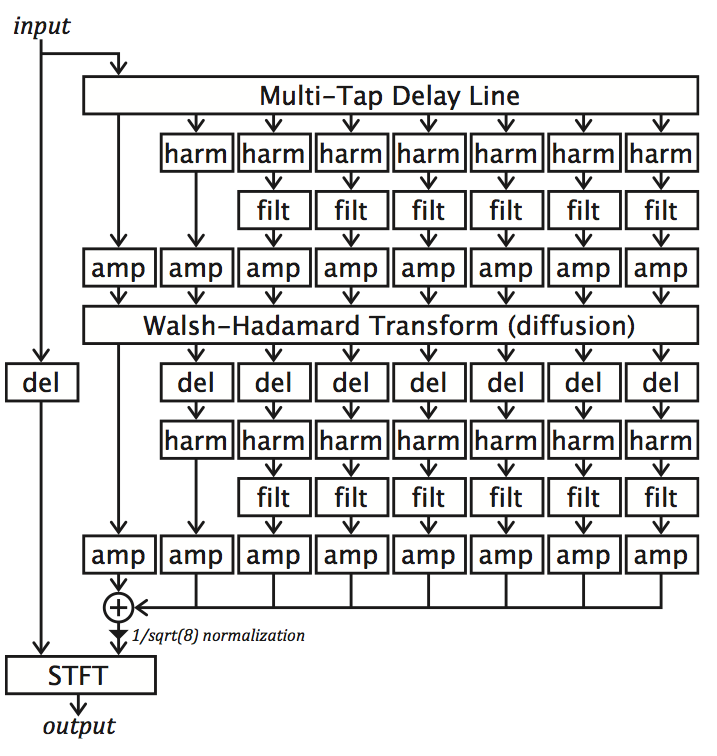
\includegraphics[width= 9cm]{Structure.png}
\caption{Block diagram of the warm chorus algorithm. \cite{dudas}}
\label{fig:struct}
\end{figure}
\subsection{Harmonizer}

Harmonizer is structure which detunes input signal slightly to get different "players" play
slightly out of tune as in the real orchestra section. The block diagram of the harmonizer
is shown in figure \ref{fig_harm}

In harmonizer structure there are four channels which are windowed with four sinusoidal windows
that are 90 degrees more out of phase than previous. To decrease the beating effect that is present
in the current chorus there is added some random variance to the detuning of the sound. That means
that each window is slightly differently out of tune. That is as well related to the real world as the players
usually do not play whole music piece in same detuning. \cite{dudas}
\begin{figure}[ht]
\centering
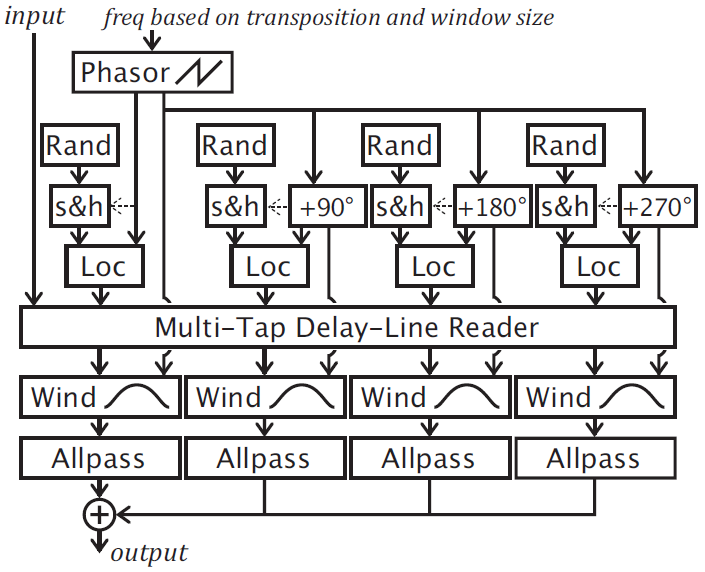
\includegraphics[width = 8cm]{harmonizer.png}
\caption{Chorus Harmonizer Block Diagram. \cite{dudas}}
\label{fig_harm}
\end{figure}

The detuning is made with multi-tap delay-line which is modulated with phasor signal which is basic sawtooth
wave form. After that each channel is windowed by using Hanning window and after that it is allpass filtered.
The windows are triggered with phasor signal and it as well triggers the randomization for each window.
After allpass fitering all the channels are summed together. \cite{dudas}


\section{Results}

\clearpage
\section{Conclusions}

Conclusions text.




% References. This is done using BibTeX and NatBib package.
% This can be used at the beginning of the seminar to present all references easily.
% Comment out when ready.
%\nocite{*} 
%\renewcommand{\refname}{\vspace{-1cm}\normalsize\section{References}}
% Select style for bibliography. Current is following Harvard-style which is usually used
% in acoustics seminars.
%\bibliographystyle{abbrvnat}
% Reference to bibliography file.
%\bibliography{refs}

\clearpage
\begin{thebibliography}{99}
\bibitem{dudas} Warm Chorus...
\end{thebibliography}

\end{document}
